\subsection{Classification} \label{subsec:classification}

\begin{figure}[h!]
    \centering
    \includegraphics[width=0.4\linewidth]{img/classify_block.png}
    \caption{Algorithm Flowchart of the Classification Subsystem}
    \label{fig:classify_algorithm_flowchart}
\end{figure}

As depicted in figure \ref{fig:classify_algorithm_flowchart} the algorithm is somewhat straight forward. In the initialization procedure first the weights of the system are obtained, later the frame is passed through the neural network to classify where there are any objects that belong to the 80 different classes or not. However, not all of these classes are important to us. Therefore, the list containing the detected classes are compared with the desired classes which are cats and dogs. If there is a dog present, the system returns the string 'dog' no matter the presence of a cat. If there are cats present, the system returns the string 'cat'. If the debug mode is activated, the algorithm puts every classified object in a box with the confidence rate written on top. It also writes the time that has passed to do this procedure to every frame. This way, it can easily be defined what the network is doing wrong so the problem is easily detected, fixed and improved. In addition to this, the algorithms contain logging info lines which log what the system is currently doing to a separate file at all times. This was when an error is encountered it can be easily avoided. 

\subsubsection{Requirements}
\begin{itemize}
    \item Differentiate between cats and dogs.
    \item Clearly recognize scenes without any dogs. 
    \item Detect how many cats are present.
    \item Have reliable confidence for the classifications.
\end{itemize}

% ===== Relation to System Level Requirements ===== %

\subsubsection{Solution}
Neural network based solution is utilized in order to detect cats and dogs. There are other methods that are considered and eliminated. The methods are mainly : 
\begin{itemize}
    \item Histogram based
    \begin{itemize}
        \item Not capable of extracting complex features.
        \item Very variant to the ambient noise.
        \item No ability to understand the object properties, just color.
        \item Very bad response to illumination, rotation, color variations in cats.
    \end{itemize}
    \item Feature descriptor
    \begin{itemize}
        \item Very hard to find appropriate data.
        \item Not accurate compared to neural networks.
        \item Difficult to develop algorithms for mass data set.
    \end{itemize}
\end{itemize}

%TODO: YOLO'dan bahset. 

After different alternatives were evaluated and discussed, neural networks, especially Convolutional Neural Networks are chosen for classification purposes. Neural networks are universal approximators according to the universal approximation theorem \cite{bib::universalApproximator}. Therefore, it is clear that, any feature can be taken into account with neural networks. Also, powerful results obtained from the CNNs in recent years \cite{cite:CNNPowerful} make it a better choice for our application. Moreover, it is easy to find a lot of different resources, not only document and articles but also the codes and ready to use trained networks. With the adoption of CNNs as the classifying method, the disadvantages of inaccuracy and complexity that exist in other methods were avoided.

A basic NN architecture can be seen in figure \ref{fig:proposedArchNN}. Inputs are not only images, but also the environmental features such as food case weight and animal weight. All of them are not going to be implemented, and most of them will be model dependent, for different applications of the product, different model features will be included. Figure shows all possible features that will be included in the neural network prediction model. More basic and simpler network architecture is given in figure \ref{fig:simpleArchNN}, the networks we are going to be using are more complex and more layered structures which are basically the same in principle but requires more work in practice.

The neural network architecture os trained, validated, and tested before it gets ready to be used. There are a lot of ready to use open source repositories which provide very powerful trained networks. Such repositories include YOLO, tensorfow pre-trained models.  There are very different implementation details which are not going to be explained in this report. 


\tikzset{%
  every neuron/.style={
    circle,
    draw,
    minimum size=1cm
  },
  neuron missing/.style={
    draw=none, 
    scale=4,
    text height=0.333cm,
    execute at begin node=\color{black}$\vdots$
  },
}
\begin{figure}[h!]
\centering
\resizebox{\linewidth}{!}{
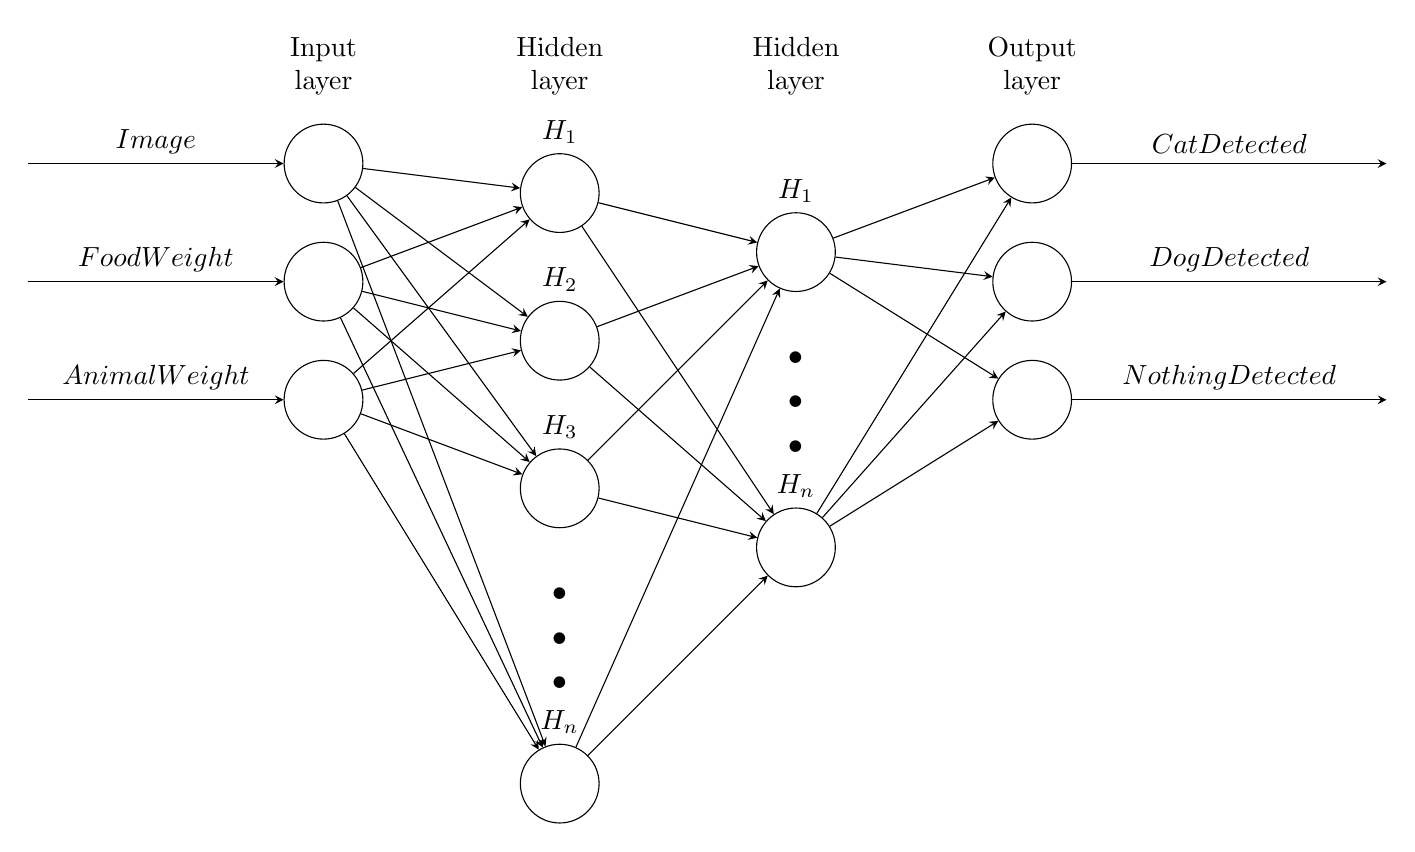
\begin{tikzpicture}[x=1.5cm, y=1.5cm, >=stealth]

% missing = 3 nokta
\foreach \m/\l [count=\y] in {1,2,3}
  \node [every neuron/.try, neuron \m/.try] (input-\m) at (0,2.5-\y) {};

\foreach \m [count=\y] in {1,2,3,missing,4}
  \node [every neuron/.try, neuron \m/.try ] (hidden1-\m) at (2,2.5-\y*1.25) {};

\foreach \m [count=\y] in {1,missing,2}
  \node [every neuron/.try, neuron \m/.try ] (hidden2-\m) at (4,2-\y*1.25) {};

\foreach \m [count=\y] in {1,2,3}
  \node [every neuron/.try, neuron \m/.try ] (output-\m) at (6,2.5-\y) {};

% writings
\draw [<-] (input-1) -- ++(-2.5,0)
node [above, midway] {$Image$};
\draw [<-] (input-2) -- ++(-2.5,0)
node [above, midway] {$Food Weight$};
\draw [<-] (input-3) -- ++(-2.5,0)
node [above, midway] {$Animal Weight$};

\foreach \l [count=\i] in {1,2,3,n}
  \node [above] at (hidden1-\i.north) {$H_\l$};

\foreach \l [count=\i] in {1,n}
  \node [above] at (hidden2-\i.north) {$H_\l$};

\draw [->] (output-1) -- ++(3,0)
node [above, midway] {$Cat Detected$};

\draw [->] (output-2) -- ++(3,0)
node [above, midway] {$Dog Detected$};

\draw [->] (output-3) -- ++(3,0)
node [above, midway] {$Nothing Detected$};


% arrows for connections
\foreach \i in {1,...,3}
  \foreach \j in {1,...,4}
    \draw [->] (input-\i) -- (hidden1-\j);

\foreach \i in {1,...,4}
  \foreach \j in {1,...,2}
    \draw [->] (hidden1-\i) -- (hidden2-\j);

\foreach \i in {1,...,2}
  \foreach \j in {1,...,3}
    \draw [->] (hidden2-\i) -- (output-\j);

\foreach \l [count=\x from 0] in {Input, Hidden, Hidden, Output}
  \node [align=center, above] at (\x*2,2) {\l \\ layer};

\end{tikzpicture}
}
\caption{Proposed Neural Network Architecture}
\label{fig:proposedArchNN}
\end{figure}


\tikzstyle{block}=[fill=white,draw=red,minimum size=1.5cm, rounded  corners,align=center]
\begin{figure}[h!]
\centering
\resizebox{\linewidth}{!}{
 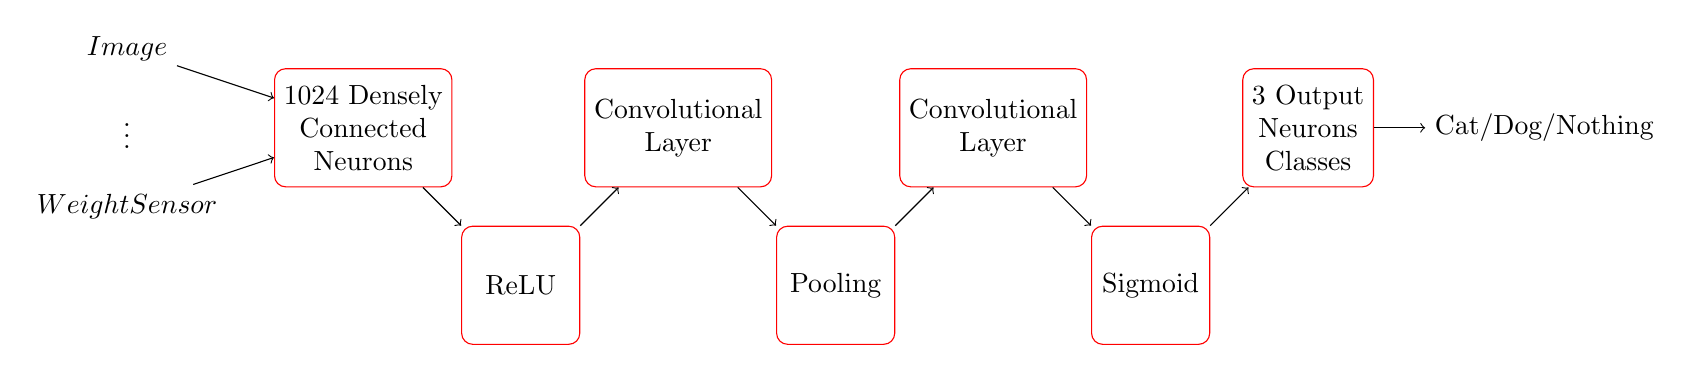
\begin{tikzpicture}
  \node[block] (dense1) {1024 Densely\\Connected\\Neurons};
  \node[draw=none, right of=dense1, node distance=2cm] (reluTop1) {};
  \node[block, below of=reluTop1, node distance=2cm] (relu1) {ReLU};
  
  \node[draw=none,left of=dense1,node distance=3cm] (feature0) {$\vdots$};
  \node[draw=none,above of=feature0,node distance=1cm] (feature1) {$Image$};
  \node[draw=none,below of=feature0,node distance=1cm] (featuren) {$WeightSensor$};
  
  \node[block,right of=reluTop1,node distance=2cm] (dense2) {Convolutional\\Layer};
  \node[draw=none, right of=dense2, node distance=2cm] (reluTop2) {};
  \node[block, below of=reluTop2, node distance=2cm] (relu2) {Pooling};
  
  \node[block,right of=reluTop2,node distance=2cm] (dense3) {Convolutional\\Layer};
  \node[draw=none, right of=dense3, node distance=2cm] (reluTop3) {};
  \node[block, below of=reluTop3, node distance=2cm] (relu3) {Sigmoid};
  
  \node[block,right of=reluTop3,node distance=2cm] (output) {3 Output\\Neurons\\Classes};
  \node[draw=none, right of=output, node distance=3cm] (outputName) {Cat/Dog/Nothing};
  
  
  \draw [->] (output) -- (outputName);
  \draw [->] (feature1) -- (dense1);
  \draw [->] (featuren) -- (dense1);
  \draw [->] (dense1)   -- (relu1);
  \draw [->] (relu1)    -- (dense2);
  \draw [->] (dense2)   -- (relu2);
  \draw [->] (relu2)    -- (dense3);
  \draw [->] (dense3)   -- (relu3);
  \draw [->] (relu3)    -- (output);
  
 \end{tikzpicture}
}
\caption{Simple Neural Network Architecture Design}
\label{fig:simpleArchNN}
\end{figure}


% ===== Algorithms, among other content, belong here ===== %

\subsubsection{Risks}

Possible risks include computation burden and false positives in the neural networks. Computation burden is the major factor in selecting and maintaining the correct hardware, consequently the cost. On the other hand, false positives play a crucial role in performance of the product. Therefore, both of these risks are going to be inspected seriously.

Computational burden is an important issue in choosing correct hardware. Since more power is demanded as computational burden increases, more weight and more complex electronic components would have been required if computations were to be done in the product. On the other hand, computational power requirement is not a big issue in servers that can do massive works in parallel. This is the actual motivation behind the server - client model exploited in this product. With the advancing product number and models, servers can provide very powerful computational capability for a very little operating cost. In Digital Ocean, 10 \$ per month can provide required computations for 30 products at the same time with the early prototype configuration requirements. In addition, improvements in the algorithm and parallel processing capabilities provided by major cloud computing platforms can increase the efficiency of the computation. Moreover, by adjusting the system properties, network - algorithm - data optimizations, 200 product computations are expected to be done on a 10 \$ machine, which makes 0.05 \$ of operating cost per month.

The other major risk of false positives, or more generally, poor performance situations encountered in regular operation risks are planned to be solved in a number of steps. Fine tuning, time dependency of consecutive frames, probabilistic models such as confidence intervals are supposed to be used in this process. These processes mainly relate to dogs classified as cats since false positives are the worst cases, and possibly they damage or misuse the system. Some methods are explained below.

The first method to be considered is to make the preprocessing stage as effective as possible. This way, the inputs to the classifier are adjusted according to the neural network's data set which reduces the error rate. This also increases the system speed and accuracy. 

The second method is fine tuning, it is the most basic and important process in the improvement of the classification performance. Since the models used are trained on online data sets and mainly in good ambient conditions, their adaptation to the Felerest product domain requires some samples, their editions, and re-training of the network \cite{cite:cnnFineTune1}. During this procedure, it is crucial not to disrupt the already existing structure of the network and the weights. To prevent this, the network's trained data set should be taken into account. The images that are to be trained with fine tuning should not be vastly different from the data set. Moreover, the quantity of the fine tuning set should not be too small and should contain some images from the actual data set. In this project 150-200 frames were seen as an optimal quantity to achieve fine tuning. Noise factors should also be taken into account when doing this. For these reasons, more research is to be conducted on the fine tuning topic. 

% TODO
%Time dependency of consecutive frames is another information that is going to be used in the design of ...

% Statistical approaches, 
% ===== Indicate alternative solutions ===== %

\subsubsection{Tests}

Some test results are given as in figure \ref{fig:catbowl}. Tests are done in extreme conditions where light is very little, and view angle is narrowed by intent. With this configuration, worst case situations are investigated. Tests are done on 3 different real cats and 20 cat, 10 dog photos. The results are astonishing, for 50 samples taken from pictures of animals, only 3 pictures which is the same cat picture with a lot of effects. Overall the performance was unexpectedly high with a whooping accuracy of more than 90 percent. 

The data set is given in \href{http://dosya.afeserpi.duckdns.org:8080/dataset}{\textcolor{blue}{this link}}.The test was done on images obtained from google randomly. These images were printed on A4 paper in large scale and held in front of the camera at various angles from various distances. Because of the enlarged photos, low quality of the printer and the images itself there were some uncompensated noise factors. However the results are promising. Note that this accuracy results are only for raw images, other sensors, decision maker and other probabilistic models are not taken into account. The expected accuracy for the system to work are going to be higher than 99 \%, with very little false positives. 

% ===== Procedure and results of tests ===== %
% kamera kaymis ya, asagi bakiyor neyse
\begin{figure}[ht!]
     \centering
     \begin{subfigure}[b]{0.49\textwidth}
     \includegraphics[width=\linewidth]{img/catbowl.jpg}
     \caption{}
     \label{fig:catbowl1}
     \end{subfigure}
     \begin{subfigure}[b]{0.49\textwidth}
     \includegraphics[width=\linewidth]{img/catbowl2.jpg}
     \caption {}
     \label{fig:catbowl2}
     \end{subfigure}        
     \begin{subfigure}[c]{0.49\textwidth}
     \includegraphics[width=\linewidth]{img/catbowl3.jpg}
     \caption {}
     \label{fig:catbowl3}
     \end{subfigure}      
     \caption{Images of real life  test results}
     \label{fig:catbowl}
\end{figure}

% ===== Justification of requirements ===== %

% ===== Comparison with alternative solutions ===== %

% ===== Error sources, their impact and ways to mitigate ===== %

\subsubsection{Plans}

\begin{itemize}
    \item Conduct extensive research on fine tuning. 
    \item Conduct extensive research on pre-processing. 
    \item Examine the training data set of the original network for better implementation of fine tuning. 
    \item Detect how many cats are present in a single frame. 
    \item Implement fine-tuning and preprocessing into classification module. 
    \item Improve speed, optimize the code further. 
\end{itemize}

% ===== State names of responsible person/people ===== %

\subsubsection{Anticipated Difficulties}

In the following parts of the classification system, it is expected to encounter further difficulties regarding the speed of the system. This is because the classification module rely on the computation power strongly. After it has been implemented to the rest of the system the time for the camera to open, the time for the frame to pass through the preprocessing module, the image complexity, the constant stream of data the will surely slow down the system. Another issue that was already encountered was after the implementation of the whole system, the camera was driving too much power that the PWM signals going to other parts of the overall system were disrupted. This caused the sensors and the motor to malfunction. To avoid this in the future an Arduino is to be used for better PWM signals with less noise. This is crucial since back-end and identification rely strongly on the speed of the classification part. More information on this is presented in the electronics subsystem section. Another anticipated difficulty is the weights to be more inaccurate after fine tuning. This is due to the unfamiliarity to this technique and somewhat complexity of it. Therefore, the plan is to approach it cautiously after extensive research. 

\subsubsection{Test Plans}

\begin{itemize}
    \item Compare the confidences, speed, accuracy between the fine tuned data and the original network.
    \item Test with real cats and dogs.
    \item Test with multiple cats by putting a picture. 
    \item Test the system's confidence, speed and accuracy before preprocessing and after preprocessing by running the same test data set. 
\end{itemize}

% ===== Measure of success ===== %

